\chapter{Direct-Current Circuits}

Now we shall look in more detail at electrical circuits, which have a network of conductors and other devices connected together. Generally, the conductors can be idealized as thin wires, each of which carries a constant current in a stationary situation, and junctions where all the incoming currents get divided up into all the outgoing currents, with no charge of either sign building up at the junction. This was given by \textbf{Kirchhoff's junction rule} or \textbf{current law} or \textbf{first law: Sum of currents into a junction is zero}.

Since in a stationary situation the electric force is a \textbf{conservative force}, with a \textbf{potential} (potential energy per charge, measured in the SI unit of $\SI{1}{V} = \SI{1}{J/C}$) that is defined up to one overall additive constant (so that the potential differences or voltages between two points are uniquely defined), we get \textbf{Kirchhoff's loop rule} or \textbf{voltage law} or \textbf{second law: the algebraic sum of potential differences around any closed loop is zero} (the algebraic sum means keeping track of signs. If we have a potential increase from $a$ to $b$, so $V_b - V_a = V_{ba} = -V_{ab} > 0$, the potential difference is positive; if $V_b < V_a$, $V_b - V_a = V_{ba} = -V_{ab} < 0$, this is negative).

Now let us use Kirchhoff's rules to get the effective resistance $R_\text{eff}$ of $N$ resistors, of resistances $R_i$ with $i$ running from 1 to $N$, that is, $R_1, R_2, \ldots, R_N$, when the resistors are connected in \textbf{series} and in \textbf{parallel}. In series, we have 
\begin{equation}
R_\text{eff} = R_\text{eq} = \sum R_i = R_1 + R_2 + \cdots + R_N.
\end{equation}
In parallel, we have
\begin{equation}
\dfrac{1}{R_\text{eff}} = \dfrac{1}{R_\text{eq}} = \sum \dfrac{1}{R_i} = \dfrac{1}{R_1} + \dfrac{1}{R_2} + \cdots + \dfrac{1}{R_N}.
\end{equation}

A wire of cross section $A$ can be considered as a parallel arrangement of wires of cross sections adding up to $A$, which fits $\frac{1}{R} = \frac{A}{\rho L} = \frac{\sigma}{L}A$, adding up the $A$'s.

\section{Electrical Measuring Instruments}
Electrical measuring instruments for current (\textbf{ammeters}), potential difference or voltage (\textbf{voltemeters}), and resistance (\textbf{ohmmeters}) generally have a basic unit for measuring current, such as a \textbf{d'Arsonval galvanometer}. This meter has a coil of wire on a pivot that is in a magnetic field of a permanent magnet that is also part of the meter. The coil has a spring attached to it that supplies a restoring force when the coil is twisted away from its equilibrium position (since this force tries to restore the \textbf{orientation} of the coil, with its center at a fixed \textbf{position,} what is more relevant is the restoring \textbf{torque} of the spring). When a current passes through the coil, the magnetic field exerts a torque proportional to the current. Therefore, after the coil settles down to a fixed orientation (due to frictional torque, so that the system is like a damped harmonic oscillator for orientation) the restoring torque (generally approximately proportional to the angle of the coil orientation relative to the equilibrium orientation) balances the torque produced by the magnetic field on the current in the coil (which is proportional to the current). Thus the angle that the coil has twisted from its equilibrium orientation is approximately proportional to the current in the coil and thus gives a measure of that current. A pointer needle attached to the coil then gives a reading on a calibrated scale (even if the angle of twist is not very precisely proportional to the current, during manufacture one can use currents otherwise calibrated to calibrate the scale of the meter).

An \textbf{ammeter} uses such a d'Arsonval galvanometer directly to measure the current through it. If one has a circuit element with current running through it that one wishes to measure, one needs to break the circuit and attach the two separated ends to the two terminals of the ammeter, so that the current that was just running through the circuit now runs through the ammeter and is measured by it.

Of course, inserting an ammeter into a circuit adds the additional resistance of the ammeter to the circuit and thus reduces the current reading from what it actually was in the circuit without the ammeter inserted into it. To minimize this error of the ammeter reading, we want the ammeter resistance as \textbf{low} as possible, but unless we use superconducting coils at very low temperatures, there is a practical limitation of how low the resistance can be.

For an ammeter to be able to measure a larger range of currents, it may have a \textbf{shunt resistor} that can be put in \textbf{parallel} to the coil, so that a larger total current can pass through the complete ammeter (coil plus resistor) than what would give a full-scale deflection of the coil if all of the current passed through the coil. For example, suppose $I_\text{fs}$ is the current passing through the coil that would give full-scale deflection, but one wants to be able to measure currents up to $I_a$ passing through the full ammeter, so that $I_\text{fs}$ passes through the coil with resistance $R_c$, and $I_a - I_\text{fs}$ passes through the shunt with resistance $R_\text{sh}$:

\begin{figure}[h]
\centering
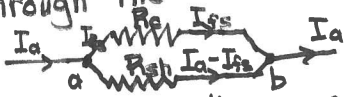
\includegraphics[width=0.4\textwidth]{shunt.png}
\end{figure}

Since the voltage drop $V_{ab} = I_\text{fs}R_c = (I_a - I_\text{fs})R_\text{sh}$, so with $R_c$ fixed, we need $R_\text{sh} = \frac{I_\text{fs}R_c}{I_a - I_\text{fs}}$. Shunts of \textbf{decreasing} resistances $R_\text{sh}$ then allow an ammeter to measure increasing currents $I_a$.

A \textbf{voltmeter} is designed to measure the potential difference or voltage $V_{ab} = V_a - V_b$ between two points in a circuit that one connects the two terminals of the voltmeter to without breaking the circuit as one does with an ammeter. In other words, a voltmeter leaves the original circuit intact and provides a parallel path for a tiny amount of current to pass through it to deflect the coil and give a meter reading. To avoid having a large amount of current passing through it (which would increase the voltage drop in other parts of the circuit not parallel to the voltmeter and hence make the voltage measured across the voltmeter lower than what it would be if the voltmeter were not attached), one wants the voltmeter resistance to be as \textbf{high} as possible, though it must be low enough to give enough current through the coil that one can get a meter reading.

\begin{figure}[h]
\centering
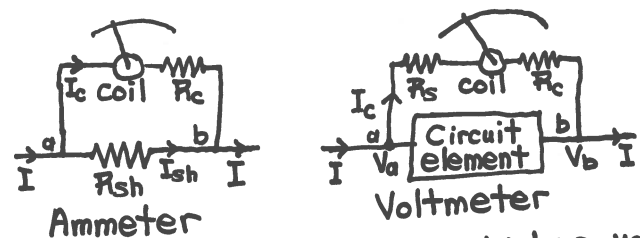
\includegraphics[width=0.8\textwidth]{ammetervoltmeter.png}
\end{figure}

To be able to measure higher voltages tha nwhat would give full-scale deflection with just the coil resistance $R_c$ (which with the full-scale current $I_\text{fs}$ would be a voltage of $V_0 = I_\text{fs}R_c$), one can include in the voltmeter an additional resistance $R_s$ in \textbf{series} with the coil, so that then a full-scale deflection at current $I_\text{fs}$ would occur for a voltage of $V_v = I_\text{fs}(R_c + R_s) = V_0\bracks{ 1 + \frac{R_s}{R_c} }$. Resistors in a series of \textbf{increasing} resistances $R_s$ then allow a voltmeter to measure increasing voltages $V_v$.

Thus with a resistor $R_s$ in series with that of the coil ($R_c$), a voltmeter has a total resistance $R_v = R_c + R_s$, whereas with a shunt resistor $R_\text{sh}$ in parallel with the coil $R_c$, an ammeter has resistance $\frac{1}{R_A} = \frac{1}{R_c} + \frac{1}{R_\text{sh}}$.

Suppose we originally have the circuit at the bottom, with a source of emf $\varepsilon$ and internal resistance $r$ in series with a resistance $R$. The total resistance is $R + r$, so in this situation the current is $I_0 = \frac{\varepsilon}{R + r}$. The total power produce by the emf (not counting the negative power produce by the internal resistance $r$) is $I_0\varepsilon = \frac{\varepsilon^2}{R+r}$. The power dissipated in the internal resistance is the current through it, $I_0$ (the same everywhere around this simple circuit of one loop), multiplied by the voltage drop through $r$, which is $I_0r$, so the product is $I_0^2r = \frac{\varepsilon^2r}{(R+r)^2}$.

The power delivered to the external resistance $R$ is $I_0^2R = \frac{\varepsilon^2R}{(R+r)^2}$. We can then check that the total power dissipated both internally and externally is $I_0^2r + I_0^2R = I_0^2(r+R) = \frac{\varepsilon^2(r+R)}{(R+r)^2} = \frac{\varepsilon^2}{R + r}$, which matches the power generated, $I_o\varepsilon = \frac{\varepsilon^2}{R+r}$. Assuming $r$ is fixed, if we change the external resistance $R$, the total power dissipated, $\frac{\varepsilon^2}{R+r}$, is a monotonically decreasing function of $R$ and so is maximized when $R$ is minimized, say to $R=0$ when the two terminals of the source of emf are connected together with no resistor. This ``shorts out" the source of emf, and if $r$ is low enough, this can give a high enough current $I_{0_\text{max}} = \frac{\varepsilon}{r}$ and power $P_\text{max} = \dfrac{\varepsilon^2}{r}$ to wreck a battery or perhaps even to start a fire.

Suppose we do not want to maximize the total power dissipated by both resistors, but just the power delivered to the external resistor $R$ to be dissipated there (turned into heat), $P_\text{ext} = \frac{\varepsilon^2R}{(R+r)^2}$, with $r$ kept fixed. This maximum occurs where 
\begin{align*}
\dfrac{\di}{\di R} P_\text{ext} &= \varepsilon^2 \sbracks{ \dfrac{\di}{\di R} \dfrac{R}{(R+r)^2} } \\
&= \varepsilon^2 \dfrac{r-R}{(R+r)^3} = 0,
\end{align*}
hence the maximum power that source of emf $\varepsilon$ with internal resistance $r$ can deliver to an external resistance $R$ whose magnitude can be varied is $\frac{\varepsilon^2}{4r}$.

Now let us add an ammeter and a voltmeter to the circuit to try to measure the current $I_0$, resistance $R$, voltage $V_{ac} = I_0R$ across the resistor, and power $I_0V_{ac} = I_0^2R$ dissipated by the resistor. If the ammeter had zero resistance, $R_A = 0$, it would not add to the resistance of the rest of the circuit that it is in series with, and if the voltmeter and infinite resistance, $R_V = \infty$, it would not decrease the resistance of the part of the circuit where it is in parallel with the original circuit, so in this case the measured current would indeed be $I=I_0$, and the measured voltage across $R$ would indeed by $V= I_0R$, so one could get $I_0 = I$, $V_{ab} = V$, $R = \frac{V}{I}$, and $P_\text{ext} = IV$. But with an actual ammeter with $R_A > 0$, and an actual voltmeter with $1/R_v > 0$, things are a bit different.

With nonzero resistance of the ammeter and the nonzero current through the voltmeter (due to the fact that it does not have infinite resistance), they do not read the same current and voltage as would be present in their absence. 

\section{Ohmmeters}

An \textbf{ohmmeter} is used to measure resistance directly of an electrical device that is passive (no source of emf within it) and is not connected to as circuit with current flowing (not counting the circuit formed by connecting the device to the ohmmeter. The ohmmeter has its own source of emf within it (ex. a battery) unlike an ammeter or voltmeter that uses the current or voltage produced by an external source of emf. 

An ohmmeter has a source of emf $\varepsilon$, a d'Arsonaval galvanometer to measure the current (and so acting like an ammeter though without any shunt resistance), and a variable resistance $R_s$. First, the two terminals are connected together and $R_s$ set to give full-scale deflection. Then, the two terminals are placed at opposite ends of the resistance $R$ to be measured, so the total resistance becomes $R_s + R$. Therefore, when the two terminals of the ohmmeter are connected together with only the resistance $R_s$, $I_0 = I_\text{fs} = \frac{\varepsilon}{R_s}$. Then when the resistance $R$ is added to the circuit, the meter reads $\frac{\varepsilon}{R_s + R} = \frac{R_sI_\text{fs}}{R_s + R}$, giving $R = R_s\bracks{ \frac{I_\text{fs}}{I} - 1 }$. The scale on the meter gives $\frac{I_\text{fs}}{I}$, which with known $R_s$ (from the way the meter is constructed) one can measure $R$.

Because there is no other source of emf giving a current through the resistor $R$ other than the emf in the ohmmeter, its measurement of $R$ directly gives the correct value, unlike the current measured by an ammeter of positive resistance and by a voltmeter of non-infinite resistance.

Unlike a voltmeter, a \textbf{potentiometer} can measure the emf of a source without drawing any current that would change the voltage across it and its internal resistance. The potentiometer has a source of emf $\varepsilon_1$ that produces a nonzero current $I_1$ through the bottom loop of total resistance $R_{ab} + r_1$, so $I_1 = \frac{\varepsilon_1}{R_{ab}+r_1}$. The potentiometer also includes the d'Arsonval galvanometer between terminal $d$ and a point $c$ that can be moved along the resistor $R_{ab}$ to give a resistance $R_{cb} = \frac{cb}{ab}R_{ab}$ proportional to the length $cb$. This length, and hence $R_{cb}$, is adjusted until the galvanometer reads zero current $I = 0$ in the top loop, where the source of emf $\varepsilon$ and its internal resistance have terminals $b$ and $d$ attached to the potentiometer. With $I=0$, $V_{cb} = \varepsilon$. But $V_{cb} = I_1R_{cb} = \frac{\varepsilon_1}{R_{ab} + r} \frac{cb}{ab} R_{ab}$, giving $\varepsilon$.

\section{R-C Circuits}

We now consider a nonstationary (time-dependent) situation in which we have two capacitor plates on which opposite charges can be a function of time, $+q(t)$ on one side and $-q(t)$ on the other. We also have a time-dependent current $i(t) = \frac{\di q}{\di t}$ flows into the capacitor on one side. On the opposite side, $i'(t) = -\frac{\di q}{\di t}$ flows in, so what flows out is again $i(t) = \frac{\di q}{\di t}$. 

\begin{figure}[h]
\centering
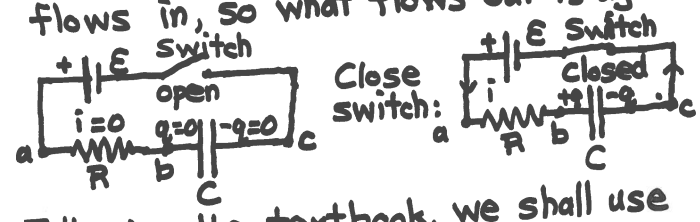
\includegraphics[width=0.7\textwidth]{switch.png}
\end{figure}

Following the textbook, we shall use lowercase $q$, $i$, and $v$ for time-dependent charge ($+q$ on the left side of the capacitor of capacitance $C$, $-q$ on the right side), current $i(t) = \dfrac{\di q(t)}{\di t}$, and voltage. When the time dependence is slow compared with the speed of light, the electric force is very nearly conservative, $\vec{E} \approx -\vec{\nabla}V$, and Kirchhoff's loop law applies.

After the switch is closed, $q(t)$ increases, so $i(t) > 0$. $V_{ab} = V_a - V_b = iR$, $V_{bc} = \frac{q}{C}$, and $V_{ca} = -\varepsilon$ through the source of emf, so Kirchhoff's loop law says $0 = V_{ab} + V_{bc} + V_{ca} = Ri + \frac{q}{C} - \varepsilon = R\frac{\di q}{\di t} + \frac{1}{C}q - \varepsilon$. This is a linear 1st-order differential equation, which we can solve by separation of variables. Thus, we have
\begin{equation}
\boxed{ q = C\varepsilon\bracks{1 - e^{-t/RC}}. }
\end{equation}
Then the current is
\begin{equation}
\boxed{ i = \dfrac{\varepsilon}{R}e^{-t/RC} = I_0 e^{-t/RC}, }
\end{equation}
where $I_0 = \frac{\varepsilon}{R}$ is the current right after the switch is closed, at $t = 0$, when $e^{-t/RC} = e^0 = 1$. Let's check that this satisfies Kirchhoff's loop law:
\begin{align}
0 &\stackrel{?}{=} Ri + \dfrac{q}{C} - \varepsilon \\
&= R\dfrac{\varepsilon}{R}e^{-t/RC} + \varepsilon\bracks{ 1 - e^{-t/RC} } - \varepsilon \\
&= \varepsilon\bracks{ e^{-t/RC} + 1 - e^{-t/RC} - 1 } \\
&= 0.
\end{align}

When $t$ gets much larger than the \textbf{time constant} $\tau = RC$ (crudely, $\frac{t}{\tau}$ ``goes to $\infty$"), $e^{-t/RC} = e^{-t/\tau} \rightarrow 0$, so $q \rightarrow Q_f = C\varepsilon$, $i \rightarrow 0$. Then $V_{ab} = iR = 0$, $V_{bc} = \dfrac{Q_f}{C} = \dfrac{C\varepsilon}{C} = \varepsilon$, and $V_{ca} = -\varepsilon$. In contrast, at the initial time, $t=0$, $q=0$ but $i = I_0 = \frac{\varepsilon}{R}$, so $V_{ab} = iR = \varepsilon$, $V_{bc} = \frac{q}{C} = 0$, and $V_{ca} = -\varepsilon$. The time constant $\tau = RC$ is also called the \textbf{relaxation constant}.

After reaching the steady-state situation (after a very long time $t >> \tau = RC$ of charging) with $I = 0$ and $q = Q_f = \varepsilon$ on the left plate, suppose we through the switch to get a new circuit bypassing the emf. Then still $V_{ab} = iR$ and $V_{bc} = \frac{q}{C}$, but $V_{ca} = 0$, so $Ri + \frac{q}{C} = R\frac{\di q}{\di t} + \frac{q}{C} = 0$, showing that $i = -\frac{q}{RC}$ is now negative (positive current now flowing clockwise around the circuit). Then $\frac{\di q}{\di t} = -\frac{q}{RC}$, $\di q = -\frac{q}{RC} \di t$, $\frac{\di q}{q} = -\frac{\di t}{RC}$, $\int\frac{\di q}{q} = \ln(q) + \text{const} = -\frac{t}{RC}$. If we reset the time to $t = 0$ when we throw this switch, then at $t=0$, $\ln(q) + \text{const} = \ln(q) - \ln(Q_f) = \ln\bracks{\frac{q}{Q_f}}$. Since now $Q_f$ is the initial charge, call it $Q_0$.

Thus, while discharging through the resistor (but with no emf in the circuit) with $q = Q_0$ at the reset $t=0$, we get $\ln\bracks{\frac{q}{Q_0}} = -\frac{t}{RC}$. Exponentiating both sides, we get
\begin{equation}
\boxed{ q = Q_0 e^{-t/RC}, }
\end{equation}
and
\begin{equation}
\boxed{ i = \dfrac{\di q}{\di t} = -\dfrac{Q_0}{RC}e^{-t/RC}. }
\end{equation}
In this case, both the charge $q(t)$ and the current $i(t)$ exponentially decrease toward zero with the same time constant $\tau = RC$, but their coefficients are different, so $\frac{i}{q} = -\frac{1}{RC} = -\frac{1}{\tau}$. $V_{ab} = iR = -\frac{Q_0}{C} e^{-t/RC}$, $V_{bc} = \frac{q}{C} = \frac{Q_0}{C} e^{-t/RC}$, $V_{ab} + V_{bc} = 0$.
\begin{figure}[h]
\centering
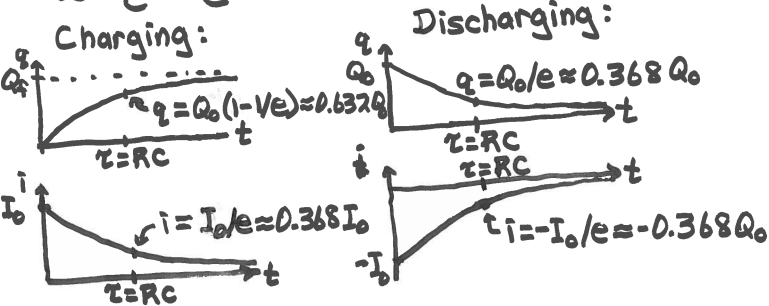
\includegraphics[width=0.7\textwidth]{charging.png}
\end{figure}